\documentclass[a4paper,oneside,12pt]{extreport}

\usepackage{mmap}
\usepackage[T2A]{fontenc}
\usepackage[utf8]{inputenc}
\usepackage[english,russian]{babel}


% Текст отчёта следует печатать, соблюдая следующие размеры полей:
% левое — 30 мм, правое — 15 мм, верхнее и нижнее — 20 мм.
\usepackage[left=20mm, right=15mm, top=15mm, bottom=15mm]{geometry}

% \setlength{\parindent}{1.25cm} % Абзацный отступ

\usepackage{setspace}
%\onehalfspacing % Полуторный интервал

\frenchspacing % Равномерные пробелы
\usepackage{indentfirst} % Красная строка

\usepackage{microtype}
\sloppy

\usepackage{titlesec}
\titlespacing*{\chapter}{0pt}{-30pt}{8pt}
\titlespacing*{\section}{\parindent}{*4}{*4}
\titlespacing*{\subsection}{\parindent}{*4}{*4}
\titleformat{\chapter}{\LARGE\bfseries}{\thechapter}{20pt}{\LARGE\bfseries}
\titleformat{\section}{\Large\bfseries}{\thesection}{40pt}{\Large\bfseries}

\usepackage{graphicx}
\usepackage{caption}

\usepackage[unicode,pdftex]{hyperref}
\hypersetup{hidelinks}

%% title begin
\usepackage{wrapfig}

\makeatletter
	\def\vhrulefill#1{\leavevmode\leaders\hrule\@height#1\hfill \kern\z@}
\makeatother
%% title end

%% begin code
\usepackage{listings}
\usepackage{xcolor}

\lstset{
	basicstyle=\footnotesize\ttfamily,
	breakatwhitespace=true,
	breaklines=true,
	commentstyle=\color{gray},
	frame=single,
	keywordstyle=\color{blue},
	stringstyle=\color{red},
	tabsize=8
}

\lstdefinestyle{lispinline}{
	frame=none,
	language=Lisp
}

\newcommand{\code}[1]{\texttt{#1}}
%% end code

%% begin theorem
\usepackage{amsthm}

\makeatletter
\newtheoremstyle{indented}
	{}% measure of space to leave above the theorem
	{}% measure of space to leave below the theorem
	{}% name of font to use in the body of the theorem
	{\parindent}% measure of space to indent
	{\bfseries}% name of head font
	{.}% punctuation between head and body
	{ }% space after theorem head; " " = normal interword space
	{}% header specification (empty for default)
\makeatother

\theoremstyle{indented}

\newtheorem{definition}{Определение}[section]
\newtheorem{example}{Пример}[section]
\newtheorem{theorem}{Теорема}[section]
\newtheorem{task}{Задание}

\makeatletter
\DeclareRobustCommand\bfseriesitshape{%
	\not@math@alphabet\itshapebfseries\relax
	\fontseries\bfdefault
	\fontshape\itdefault
	\selectfont
}
\makeatother

\DeclareTextFontCommand{\textbfit}{\bfseriesitshape}
\DeclareTextFontCommand{\define}{\bfseriesitshape}
%% end theorem

%% begin columns
\usepackage{etoolbox,refcount}
\usepackage{multicol}

\newcounter{countitems}
\newcounter{nextitemizecount}
\newcommand{\setupcountitems}{%
	\stepcounter{nextitemizecount}%
	\setcounter{countitems}{0}%
	\preto\item{\stepcounter{countitems}}%
}
\makeatletter
\newcommand{\computecountitems}{%
	\edef\@currentlabel{\number\c@countitems}%
	\label{countitems@\number\numexpr\value{nextitemizecount}-1\relax}%
}
\newcommand{\nextitemizecount}{%
	\getrefnumber{countitems@\number\c@nextitemizecount}%
}
\newcommand{\previtemizecount}{%
	\getrefnumber{countitems@\number\numexpr\value{nextitemizecount}-1\relax}%
}
\makeatother
\newenvironment{AutoMultiColItemize}{%
	\ifnumcomp{\nextitemizecount}{>}{3}{\begin{multicols}{2}}{}%
		\setupcountitems\begin{itemize}}%
		{\end{itemize}%
		\unskip\computecountitems\ifnumcomp{\previtemizecount}{>}{3}{\end{multicols}}{}}
\makeatother
\newenvironment{AutoMultiColEnumerate}{%
	\ifnumcomp{\nextitemizecount}{>}{3}{\begin{multicols}{2}}{}%
		\setupcountitems\begin{enumerate}}%
		{\end{enumerate}%
		\unskip\computecountitems\ifnumcomp{\previtemizecount}{>}{3}{\end{multicols}}{}}
%% end columns



\begin{document}

\begin{titlepage}
	{\large % 14pt instead of 12pt
	\onehalfspacing
	\centering

	\begin{wrapfigure}[7]{l}{0.14\linewidth}
		\vspace{3mm}
		\hspace{-10mm}
		
\includegraphics[width=\linewidth]{img/b_logo}
		% \includegraphics[width=0.93\linewidth]{inc/img/bmstu-logo}
	\end{wrapfigure}
	{\singlespacing \footnotesize \bfseries Министерство науки и высшего образования Российской Федерации\\Федеральное государственное бюджетное образовательное учреждение\\высшего образования\\<<Московский государственный технический университет\\имени Н.~Э.~Баумана\\ (национальный исследовательский университет)>>\\(МГТУ им. Н.~Э.~Баумана)\\}

	\vspace{-2.2mm}
	\vhrulefill{0.9mm}\\
	\vspace{-7.5mm}
	\vhrulefill{0.2mm}\\
	\vspace{2mm}

	{\doublespacing \small \raggedright ФАКУЛЬТЕТ \hspace{5mm} \underline{«Информатика и системы управления»}\\
	КАФЕДРА \hspace{10mm} \underline{«Программное обеспечение ЭВМ и информационные технологии»}\\}

	\vspace{20mm}

	\begin{center}
		\noindent\begin{minipage}{1.2\textwidth}\centering
			\textbf{ОТЧЕТ ПО ЛАБОРАТОРНОЙ РАБОТЕ №18,19}\newline
			\textbf{По курсу: "Функциональное и Логическое программирование"}\newline\newline\newline
		\end{minipage}
	\end{center}

	\vspace{20mm}

	\noindent ~~Тема \underline{~~~~~~~~~~~~~~~~~~~~~~~~~~Рекурсия в прологе.~~~~~~~~~~~~~~~~~~~~~~~~~~~~~~~~~~~~~~~~~~~}\newline
	\noindent ~~Группа \underline{~~~~~~~~~~~~~~~~~~~~~~~~~~~~~~~~~~~ИУ7-63Б~~~~~~~~~~~~~~~~~~~~~~~~~~~~~~~~~~~~~~~~~~~~~~~~~}\newline
	\noindent ~~Студент \underline{~~~~~~~~~~~~~~~~~~~~~~~~~~~~Сукочева А.~~~~~~~~~~~~~~~~~~~~~~~~~~~~~~~~~~~~~~~~~~~~~~~~~~}\newline
	\noindent ~~Преподаватель \underline{~~~~~~~~~~~~~~~~~Толпинская Н.Б.~~~~~~~~~~~~~~~~~~~~~~~~~~~~~~~~~~~~~~~~~~~~~}\newline
	\noindent ~~Преподаватель \underline{~~~~~~~~~~~~~~~~~~Строганов Ю. В.~~~~~~~~~~~~~~~~~~~~~~~~~~~~~~~~~~~~~~~~~~~~}\newline


	\begin{center}
		\vfill
		Москва~---~\the\year
		~г.
	\end{center}
	}



\end{titlepage}

\setcounter{page}{2}

\section*{Практическая часть}

\begin{task}
    Напишите 

    \begin{lstlisting}[language=Lisp]
(defun check-border (x a b)
    (and (>= x a) (<= x b)) )

(defun select-between (lst a b)
    (cond ((null lst) ())
    ((symbolp (car lst)) (cons (car lst) (select-between (cdr lst) a b)))
    ((listp (car lst)) (cons (select-between (car lst) a b) (select-between (cdr lst) a b)))
    ((check-border (car lst) a b) (cons (car lst) (select-between (cdr lst) a b)))
    (T (select-between (cdr lst) a b))) )
    \end{lstlisting}

    Пример использования:
    \begin{lstlisting}[language=Lisp] 
(select-between '(1 2 (a b 3 4) T c 4 6 11 5) 2 7) ;; (2 (A B 3 4) T C 4 6 5)
    \end{lstlisting}
\end{task}

\begin{task}
	Написать функцию, вычисляющую декартово произведение двух своих списков-аргументов.
	(Напомним, что $A\times B$ — это множество всевозможных пар $(a\;b)$, где $a\in A$, $b\in B$)

    \begin{lstlisting}[language=Lisp]
(defun decart-elem (lst elem)
	(cond ((null lst) ())
	(T (cons (list elem (car lst)) (decart-elem (cdr lst) elem)))) )
    \end{lstlisting}


    Пример использования:
    \begin{lstlisting}[language=Lisp]    
(decart-elem '(a b c) 'd) ;; => ((D A) (D B) (D C))
    \end{lstlisting}

    \begin{lstlisting}[language=Lisp]
(defun decart (lst1 lst2)
	(cond ((null lst1) nil)
	(T (append (decart-elem lst2 (car lst1)) (decart (cdr lst1) lst2)))) )
    \end{lstlisting}

    Пример использования:
    \begin{lstlisting}[language=Lisp]   
;; ((A D) (A E) (A F) (B D) (B E) (B F) (C D) (C E) (C F))
(decart '(a b c) '(d e f))  
    \end{lstlisting}
\end{task}

\begin{task}
    Почему так реализовано \code{reduce}, в чем причина? 

    \begin{lstlisting}[language=Lisp]
        (reduce #'+ ()) ; 0
        (reduce #'* ()) ; 1
    \end{lstlisting}
        
    $ L = (e_1 e_2 ... e_n )$

    (reduce F L) $\equiv$ (F ( ... (F (F $e_1$ initial-value) $e_2$)) ... $e_n$)

    \begin{lstlisting}[language=Lisp]
(reduce '+ '(1 2 3 4)) ;; 10
(reduce '* '(1 2 3 4)) ;; 24
    \end{lstlisting}

    Причина состоит в том, что если начальное значение при
    умножении будет равно нулю, то и результат будет равен нулю
    \begin{lstlisting}[language=Lisp]
(reduce '* '(1 2 3 4) :initial-value 0) ;; 0
    \end{lstlisting}

    В случае сложения результат будет на единицу больше, 
    что является некорректным результатом.
    \begin{lstlisting}[language=Lisp]
(reduce '+ '(1 2 3 4) :initial-value 1) ;; 11
    \end{lstlisting}
        

\end{task}

\begin{task}
	Пусть \code{list-of-list} список, состоящий из списков.
	Написать функцию, которая вычисляет сумму длин всех элементов \code{list-of-list}, т.~е. например для аргумента \code{((1 2) (3 4)) -> 4}.

    \begin{lstlisting}[language=Lisp]
(defun list-of-list-rec (lst len)
	(cond ((null lst) len)
	(T (list-of-list-rec (cdr lst) (+ len (length (car lst)) )))))

(defun list-of-list (lst)
	(list-of-list-rec lst 0))
    \end{lstlisting}

    Пример использования:
    \begin{lstlisting}[language=Lisp]    
(list-of-list '((1 2 3) (4 5))) ;; => 5
    \end{lstlisting}

    Вариант для структурированного списка:

    Примечание: +1 потому что нужно ещё учесть сам список (который дальше будет просматриваться).
    \begin{lstlisting}[language=Lisp]
(defun list-of-list-rec (lst len)
    (cond ((null lst) len)
        ((listp (car lst)) 
        (+ 1 (list-of-list-rec (car lst) 0) (list-of-list-rec (cdr lst) len))) 
        (T (list-of-list-rec (cdr lst) (+ 1 len))) ))

(defun list-of-list (lst)
    (- (list-of-list-rec lst 0) (length lst)))
     \end{lstlisting}
        
    Пример использования:
    \begin{lstlisting}[language=Lisp]  
(list-of-list '((1 2) (3 4) (5 6 (7 8) 9))) ;; => 10
    \end{lstlisting}
\end{task}

\begin{task}
    Написать функцию, возвращающую 
    квадрат смешанного стуктурированного списка.
    В результирующем списке только числа.
    \begin{lstlisting}[language=Lisp]
(defun square-lst (lst) 
	(cond ((null lst) Nil)
	((symbolp (car lst)) (square-lst (cdr lst)))
	((listp (car lst)) (append (square-lst (car lst)) (square-lst (cdr lst))))
	(T (cons (* (car lst) (car lst)) (square-lst (cdr lst)))) )) 
    \end{lstlisting}

    Пример использования:
    \begin{lstlisting}[language=Lisp]    
(square-lst '((1 2 a) 'b 3 T 4))    ;; => (1 4 9 16)
(square-lst '((((1 2 3)))))         ;; => (1 4 9)
    \end{lstlisting}
\end{task}


% \begin{figure}[ht!]
% 	\centering{
% 		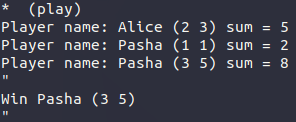
\includegraphics[width=0.5\textwidth]{img/5.png}
% 		\caption{Результат работы 5.} }
% \end{figure}

\newpage

\section*{Теоретическая часть}

\subsection*{Классификация рекурсивных функций}

\textbf{Рекурсия} -- ссылка на описываемый объект во время его описания.

\begin{enumerate}
    \item Простая - рекурсивный вызов встречается один раз.
    \item Второго порядка - несколько рекурсивных вызовов.
    \item Взаимная - несколько функций, которые могут друг друга взаимно вызывать.
    \item Хвостовая рекурсия - результат строится на входе в рекурсию.
    На выходе ничего считать не нужно.
    
    Для преобразования не хвостовой рекурсии в хвостовую можно использовать
    дополнительные параметры, в которые при каждом вызове рекурсии будет 
    формироваться и записываться результат.
    В этом случае необходимо использовать функцию-оболочку для запуска рекурсивной функции с начальными значениями дополнительных параметров.
 
    % рекурсивный вызов последний.
    \item Дополняемая рекурсия - использует дополнительную функцию.
    (результат рекурсии используется, как аргумент некоторой другой функции, которая называется дополняемой функцией)
\end{enumerate}

\end{document}